% Template file for an a0 portrait poster.
% Written by Graeme, 2001-03 based on his SOC poster.
%
% See discussion and documentation at
% <http://www.astro.gla.ac.uk/users/norman/docs/posters/> 
%
% $Id$



% We switch to portrait mode. This works as advertised.
\documentclass[a0,portrait]{a0poster}
% You might find the 'draft' option to a0 poster useful if you have
% lots of graphics, because they can take some time to process and
% display. (\documentclass[a0,draft]{a0poster})

% Switch off page numbers on a poster, obviously, and section numbers too.
\pagestyle{empty}
\setcounter{secnumdepth}{0}

% The textpos package is necessary to position textblocks at arbitary 
% places on the page.
\usepackage[absolute]{textpos}

% Graphics to include graphics. Times is nice on posters, but you
% might want to switch it off and go for CMR fonts.
\usepackage{graphics,wrapfig,times}
\usepackage{tikz}

% These colours are tried and tested for titles and headers. Don't
% over use color!
\usepackage{color}
\definecolor{DarkBlue}{rgb}{0.1,0.1,0.5}
\definecolor{Red}{rgb}{0.9,0.0,0.1}
\definecolor{applegreen}{rgb}{0.55,0.71,0.0}
\definecolor{green(ryb)}{rgb}{0.4,0.69,0.2}
\definecolor{heartgold}{rgb}{0.5,0.5,0.0}
\definecolor{oldgold}{rgb}{0.81,0.71,0.23}
\definecolor{olive}{rgb}{0.5, 0.5, 0.0}
\definecolor{yellow-green}{rgb}{0.6,0.8,0.2}

% see documentation for a0poster class for the size options here
\let\Textsize\normalsize
\def\Head#1{\noindent\hbox to \hsize{\hfil{\LARGE\color{olive} #1}}\bigskip}
\def\LHead#1{\noindent{\LARGE\color{olive} #1}\smallskip}
\def\Subhead#1{\noindent{\large\color{olive} #1}}
\def\Title#1{\noindent{\VeryHuge\color{Red} #1}}

% Set up the grid
%
% Note that [40mm,40mm] is the margin round the edge of the page --
% it is _not_ the grid size. That is always defined as 
% PAGE_WIDTH/HGRID and PAGE_HEIGHT/VGRID. In this case we use
% 15 x 25. This gives us a wide central column for text (7 grid
% spacings) and two narrow columns (3 each) at each side for 
% pictures, separated by 1 grid spacing.
%
% Note however that texblocks can be positioned fractionally as well,
% so really any convenient grid size can be used.
%
\TPGrid[40mm,40mm]{15}{25}  % 3 - 1 - 7 - 1 - 3 Columns

% Mess with these as you like
\parindent=0pt
%\parindent=1cm
\parskip=0.5\baselineskip

% abbreviations
\newcommand{\ddd}{\,\mathrm{d}}

\begin{document}

% Understanding textblocks is the key to being able to do a poster in
% LaTeX. In
%
%    \begin{textblock}{wid}(x,y)
%    ...
%    \end{textblock}
%
% the first argument gives the block width in units of the grid
% cells specified above in \TPGrid; the second gives the (x,y)
% position on the grid, with the y axis pointing down.

% You will have to do a lot of previewing to get everything in the 
% right place.

% This gives good title positioning for a portrait poster.
% Watch out for hyphenation in titles - LaTeX will do it
% but it looks awful.
\begin{textblock}{12}(0,0)
\baselineskip=3\baselineskip \Title{Unified Simplified Grapheme Acoustic
\\Modeling for Medieval Latin LVCSR}
\end{textblock}

\begin{textblock}{12}(0,1.5)
\LHead{Lili Szab{\'o}, P\'{e}ter Mihajlik, Andr\'{a}s Balog, Tibor Fegy\'{o}}
\end{textblock}

% Put logo in the top right.
\begin{textblock}{2}(13,0)
\resizebox{2\TPHorizModule}{!}{
\includegraphics{speechtex_logo.eps}}
\end{textblock}

% Introduction block.
\begin{textblock}{7}(0,3)
  \LHead{What is the problem with Latin speech recognition?}

  \begin{itemize}
      \item Latin is not spoken natively 
      \item There is no available speech database, and it is resource-heavy to create one
      \item Many variants/dialects exists, and we can only make guesses about the pronunciation
      \item The pronunciation mainly depends on
      \begin{itemize}
          \item the era of the read text 
          \item the native language of the speaker
      \end{itemize}
  \end{itemize}

\end{textblock}

% Text aquisition block.
\begin{textblock}{3}(0,6)
   \LHead{Text data}

Regions of origin: Kingdom of Bohemia (CZ), Kingdom of Hungary (HU), Kingdom of Poland (PL)

\begin{itemize}
    \item In-domain data (Monasterium): medieval charters (HU), 480k/35k token/type
    \item Background data (Latin Library): historical texts, 1.3M/115k token/type
\end{itemize}

\end{textblock}

% Alternate spellings.
\begin{textblock}{3}(4,6)
   \LHead{Spelling variants}

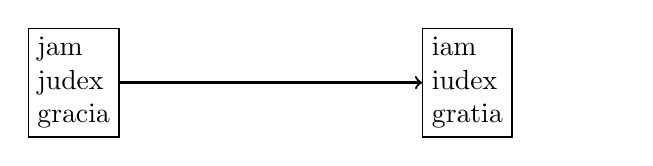
\begin{tikzpicture}
\node[draw,align=left] (corpus) at (0,0) {jam\\judex\\gracia};
\node[draw,align=left] (eval) at (5,0) {iam\\ iudex\\ gratia} (7,0);
\draw[->,thick] (corpus) -- (eval);
%\node[draw] at (0,0) {some text\\ bla bla\\ test test};
%\node[draw,align=left] at (3,0) {some text\\ spanning three lines\\ with manual line breaks};
%\node[draw,text width=4cm] at (2,-2) {some text spanning three lines with automatic line breaks};

\end{tikzpicture}

\end{textblock}

% Speech data block.
\begin{textblock}{7}(0,9)
   \LHead{Speech data}

Languages: CZ, HU, PL, RO

\end{textblock}

% Test data block.
\begin{textblock}{3}(0,11)
   \LHead{Test data}

\begin{itemize}
\item Independent medieval charters
\item Region of read text: CZ, HU, PL
\item Native language of test speakers: CZ, HU, PL, SK
\end{itemize}

\end{textblock}

% Perplexity.
\begin{textblock}{3}(4,11)
   \LHead{Perplexity measures on test}

\begin{table}
\centering
\caption{Perplexity/OOV rate}\label{tbl:perplexity}
\begin{tabular}{l|rrr|r}
\hline
& \multicolumn{3}{|c|}{Text region} & \\
\hline
Corpus & CZ & HU & PL & All \\
\hline
Monasterium & 551 & 82 & 3130 & 671 \\
Latin Library & 3266 & 3549 & 2305 & 4303 \\
Interpolated & 924 & 82 & 2288 & 953 \\
\hline
\end{tabular}
\end{table}

\end{textblock}

% LM.
\begin{textblock}{3}(0,14)
   \LHead{Language model}

\end{textblock}

% AM.
\begin{textblock}{3}(4,14)
   \LHead{Acoustic model}

\end{textblock}

% Data dimensions.
\begin{textblock}{7}(0,18)
   \LHead{Dimensions of data}

Native language of test speakers: CZ, HU, PL, SK

Region of read text: CZ, HU, PL

Speech data: CZ, HU, PL, RO

Model type: baseline, knowledge-based, USG
\end{textblock}

% Baseline.
\begin{textblock}{7}(8,3)
   \LHead{Baseline Grapheme Model}

Languages: Czech (CZ), Hungarian (HU), Polish (PL), Romanian (RO)

   \begin{itemize}
     \item All graphemes are trained
     \item Only those grapheme models are retained that are part of the Latin alphabet
   \end{itemize}

\begin{table}
%\centering
\caption{Word Error Rate (WER[\%]) results for monolingual grapheme-based acoustic models of Czech, Hungarian, Polish and Romanian (CZ, HU, PL, RO).}
\input{../../paper/tables/cz_hu_pl_ro_grapheme.tex}\label{tbl:cz_hu_pl_ro_grapheme}
\end{table}

\end{textblock}

% Source-target g2p block.
\begin{textblock}{7}(8,7)
   \LHead{Knowledge-based grapheme-to-phoneme (G2P) mapping}
  
   Languages: CZ, HU

\begin{table}
\centering
\caption{Latin digraph context-insensitive rewrite rules.}\label{tbl:digraph}
\begin{tabular}{l|rrrr}
\hline
& \multicolumn{4}{c}{Digraph} \\
\hline
   & ae & oe & ph & qu \\
\hline
CZ & e & oe & f & kv \\
HU & e & \o & f & kv \\
\hline
\end{tabular}
\vspace*{0.4 cm}
\centering
\caption{Latin context-sensitive rewrite rules. V: vowel, VP: palatal vowel, \string^VP: everything but a palatal vowel, C: consonant, $*$: zero or any, \string^: beginning of word, $[\string^stx]$: not s, t or x.}\label{tbl:context}
\begin{tabular}{l|cc|cc|cc|cc}
\hline
GR & c & c & ch & ch & gu & gu & ti & ti \\
PH & ts & k & h & k & gv & gu & tsi & ti \\
\hline
rule & \multicolumn{1}{c|}{cVP} & \multicolumn{1}{c|}{c\string^VP} & \multicolumn{1}{c|}{VC*ch} & \multicolumn{1}{c|}{\string^C*ch} & \multicolumn{1}{c|}{guV} & \multicolumn{1}{c|}{guC} & \multicolumn{1}{c|}{$[\string^stx]$tiV} & \multicolumn{1}{c|}{tiC} \\
\hline
\end{tabular}
\end{table}

\begin{table}
\parbox{.45\linewidth}{
\centering
\caption{WER[\%] for Czech-Latin source-target G2P model. Acoustic model training set: 76 hours.}
\begin{tabular}{l|rrr|r}
\hline
 & \multicolumn{3}{c}{Latin Test Text} & \\
\hline
 Speaker   &   CZ &   HU &   PL &   $\sum$ \\
\hline
 CZ        & 43.8 & 28.2 & 49.1 &     40.4 \\
 HU        & 52.0 & 40.0 & 58.7 &     50.2 \\
 PL        & 94.1 & 67.3 & 97.2 &     86.2 \\
 SK        & 30.3 & 30.0 & 44.0 &     34.8 \\
\hline
 $\sum$   & 52.8 & 38.7 & 59.6 &     50.4 \\
\hline
\end{tabular}\label{tbl:cz_phoneme}
}
\hfill
\parbox{.45\linewidth}{
\centering
\caption{WER[\%] for Hungarian-Latin source-target G2P model. Acoustic model training set: 567 hours.}
\begin{tabular}{l|rrr|r}
\hline
 & \multicolumn{3}{c}{Latin Test Text} & \\
\hline
 Speaker   &   CZ &   HU &   PL &   $\sum$ \\
\hline
CZ        & 19.4 &  \bf{6.4} & 28.0 &     17.9 \\
HU        & 25.0 & 25.4 & \bf{20.2} &     23.5 \\
PL        & 28.9 & \bf{15.4} & 41.3 &     28.5 \\
SK        & 20.4 &  \bf{9.1} & 22.9 &     17.5 \\
\hline
 $\sum$   & 22.6 & 12.5 & 28.1 &     21.1 \\
\hline
\end{tabular}
\label{tbl:hu_phoneme}
}
\end{table}

\end{textblock}


% USG block.
\begin{textblock}{7}(8,14)
	\LHead{Unified Simplified Grapheme (USG) Model}

Languages: CZ, HU, PL, RO

\begin{table}
\centering
\caption{Simplification examples for the unified model.}\label{tbl:usg-examples}
\begin{tabular}{l|rrrr}
\hline
Language & CZ & HU & PL & RO \\
\hline
Orthographic form & \v{r}ekl & \H{o}z & mi\'{s} & ap\u{a} \\
USG transcription & rekl & oz & mis & apa \\
\hline
\end{tabular}
\end{table}

\begin{table}
\parbox{.45\linewidth}{
\centering
\caption{WER[\%] for all the three-language USG models.}
\begin{tabular}{l|rrrr|r}
\hline
 & \multicolumn{3}{c}{Speaker} & \\
\hline
 AM Language   &   CZ &   HU &   PL &   SK &   $\sum$ \\
\hline
 CZ+HU+PL      & 28.2 & 28.2 & 27.7 & 22.4 &     26.6 \\
 CZ+HU+RO      & 23.3 & 21.4 & 23.9 & 19.2 &     21.9 \\
 CZ+PL+RO      & 24.6 & 33.1 & 25.6 & 19.8 &     25.8 \\
 HU+PL+RO      & 24.8 & 21.5 & 25.7 & 20.7 &     23.2 \\
\hline
\end{tabular}\label{tbl:three_language_usg}
}
\hfill
\parbox{.45\linewidth}{
\centering
\caption{WER[\%] for USG model of Czech, Hungarian, Polish and Romanian (CZ+HU+PL+RO).}
\begin{tabular}{l|rrr|r}
\hline
 & \multicolumn{3}{c}{Latin Test Text} & \\
\hline
 Speaker   &   CZ &   HU &   PL &   $\sum$ \\
\hline
CZ        & 20.4 & \bf{11.8} & 30.7 &     21.0 \\
HU        & 21.1 & \bf{14.6} & 25.7 &     20.5 \\
PL        & 23.0 & \bf{10.0} & 33.0 &     22.0 \\
SK        & 14.5 & \bf{12.7} & 24.8 &     17.3 \\
\hline
 $\sum$   & 19.9 & 12.2 & 29.0 &     20.4 \\
\hline
\end{tabular}
\label{tbl:cz_hu_pl_ro_usg}
}
\end{table}

\end{textblock}

% If you want to add a figure do something like this:

%\begin{textblock}{3}(0,15)
%  \begin{center}
%\resizebox{3\TPHorizModule}{!}{\includegraphics{my_figure.eps}}
%\\Figure 5: Googles per Snark (renormalised with wild angry men
%  \end{center}
%\end{textblock}

\begin{textblock}{9}(3.5,21.2)
\LHead{Conclusions}

\begin{itemize}
\item Four-language USG is the best
\item It is able to generalize over different speaker test sets
\end{itemize}

\end{textblock}



% Place the group logo at the bottom left - visually this balances
% well with the University logo at the top right. 
%\begin{textblock}{3}(0.1,22)
%  \begin{center}
%    Another logo here
%%\resizebox{1.5\TPHorizModule}{!}{\includegraphics{/usr/local/share/images/AandA.epsf}}
%\color{red}\\Astronomy and Astrophysics Group\\Department of Physics and
%  Astronomy\\University of Glasgow
%  \end{center}
%\end{textblock}

\end{document}

